\documentclass[12pt,a4paper]{article}
\usepackage{mathsx,tech,mytheorems}
\usepackage{tikz}
\usetikzlibrary{arrows}
\usepackage{scalalistings}\unScalaMid

\newtheorem{lemma}{Lemma}
\newtheorem{conjecture}{Conjecture}
\newtheorem{definition}{Definition}
\newtheorem{example}{Example}

\def\vec#1{\mathsf{#1}}
\def\trans#1{\stackrel{#1}\rightarrow}
\def\sqge{\sqsupseteq}
\def\sqle{\sqsubseteq}

\def\id{\mathrm{id}}
\def\params{\mathrm{params}}
%\def\srv{\vec{srvs}}
\def\fixed{\mathrm{fixed}}
\def\cpt{\vec{cpts}}
\def\cpts{\cpt}
\def\princ{\mathrm{princ}}
\def\S{\mathcal{S}}
\def\V{\mathcal{V}}

\def\improve#1{IMPROVE: \emph{#1}}
\def\impNote#1{\textbf{Implementation note:} #1}

\everymath{\it}
\sloppy

\title{Improved View Abstraction: Working Paper}
\author{Gavin Lowe}

\begin{document}
\maketitle


\def\Node{Nd}
\def\Lock{Lk}
\def\Head{Hd}
\def\Last{Lt}
\def\Con{C}
\def\InitNode{InitNd}

\section{Setting}
\label{sec:setting}

In this section, we introduce more formally the class of systems that we
consider, and our framework.  Recall that we are interested in systems with an
unbounded number of component processes, perhaps from different families,
together with some fixed processes.

We give two small examples to introduce some of the ideas.  We start with a
toy mutual exclusion example.  A resource is shared by a number of threads; a
lock is used to ensure mutual exclusion.

Each thread, with identity $me$, is modelled by a state machine, illustrated
in the top-left of Figure~\ref{fig:mutual-exclusion}.  The thread repeatedly
locks the lock, starts using the resource, ends using the resource, and
unlocks the lock.  Likewise, the lock is modelled by the state machine in the
top-right of the figure.
%
Each state comprises a \emph{control state} and zero or
more \emph{parameters}; in the case of the lock, there are two control states,
which have zero and one parameters, respectively.  Each transition is labelled
by an \emph{event}. (We use CSP-style notation in the figure; the notation
$lock?t$ indicates that the process is willing to perform any event of the
form $lock.id$, and binds the name~$t$ to the corresponding value~$id$.)
Different processes synchronise on common events; for example, the thread with
identity~$me$ will synchronise with the lock on the events $lock.me$ and
$unlock.me$.

%%%%%%%%%%%%%%%%%%%%%%%%%%%%%%%%%%%%%%%%%%%%%%%%%%%%%%%

\begin{figure}
\small
\begin{center}
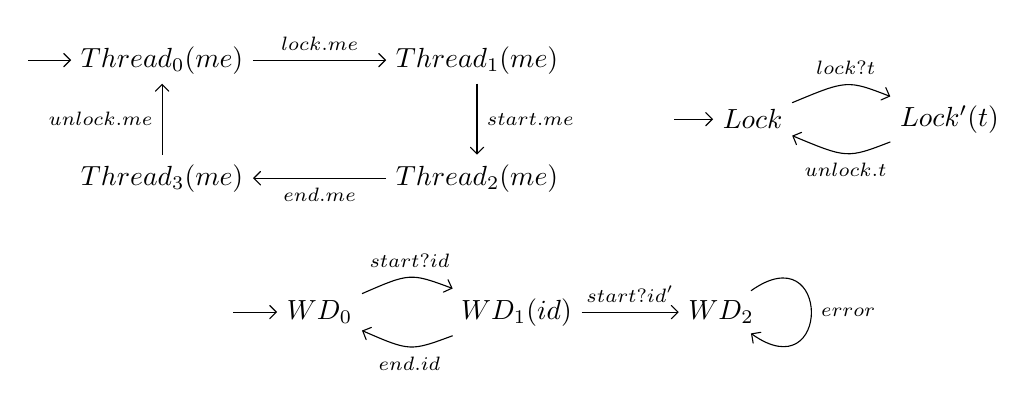
\begin{tikzpicture}[>= angle 90]
\draw (0,0) node (s0) {$Thread_0(me)$};
\path[draw, <-] (s0) -- ++(-1.7,0);
%% S1
\draw (s0) ++ (4,0) node (s1) {$Thread_1(me)$};
\path[draw, ->] (s0) -- node[above]{\scriptsize $lock.me$} (s1);
%% S2
\draw (s1) ++ (0,-1.5) node (s2) {$Thread_2(me)$};
\path[draw, ->] (s1) -- node[right]{\scriptsize $start.me$} (s2);
%% S3
\draw (s2) ++ (-4,0) node (s3) {$Thread_3(me)$};
\path[draw, ->] (s2) -- node[below]{\scriptsize $end.me$} (s3);
\path[draw, ->] (s3) -- node[left]{\scriptsize $unlock.me$} (s0);

%%%%%%%%%%%%%%%%%%%%%% Lock

\draw (s1)++(3.5,-0.75) node (lock) {$Lock$};
\path[draw, <-] (lock.west) -- ++(-0.5,0);
%% Lock'
\draw (lock)++(2.5,0) node (lock') {$Lock'(t)$};
\path[draw, ->] (lock) .. controls +(1.2,0.5) ..
  node[above]{\scriptsize $lock?t$} (lock');
\path[draw, ->] (lock') .. controls +(-1.3,-0.5) ..
  node[below]{\scriptsize $unlock.t$} (lock);

%%%%%%%%%%%%%%%%%%%%%% Watchdog

\draw (s3) ++ (2.0, -1.7) node (wd0) {$WD_0$};
\path[draw, <-] (wd0) -- ++ (-1.1,0);
%% WD1
\draw (wd0) ++ (2.5,0) node (wd1) {$WD_1(id)$};
\path[draw,->] (wd0) .. controls +(1.15,0.5).. 
  node[above] {\scriptsize $start?id$} (wd1);
\path[draw,->] (wd1) .. controls +(-1.35,-0.5).. 
  node[below] {\scriptsize $end.id$} (wd0);
%% WD2
\draw (wd1) ++ (2.6,0) node (wd2) {$WD_2$};
\path[draw, ->] (wd1) -- node[above] {\scriptsize $start?id'$} (wd2);
\path[draw,->] (wd2) .. controls +(1.4,1) and +(1.4,-1) .. 
  node[right] {\scriptsize $error$} (wd2);
\end{tikzpicture}
\end{center}
\caption{State machines for the toy mutual exclusion example.}
\label{fig:mutual-exclusion}
\end{figure}

%%%%%%%%%%%%%%%%%%%%%%%%%%%%%%%%%

The desired mutual exclusion property is captured by a \emph{watchdog},
modelled by the state machine at the bottom of
Figure~\ref{fig:mutual-exclusion}.  This observes threads starting and ending
using the resource, but performs the distinguished event $error$ if two
threads are using the resource simultaneously.  The correctness condition,
then, is that $error$ does not occur.

A system will consist of an arbitrary collection of threads, but a single lock
and a single watchdog.  Therefore we model the threads as components (each
with its own identity), but the lock and watchdog as fixed processes.
Formally, each system is parameterised by a set $ThreadID$ of thread
identities.  Each system state comprises a state for each thread $t \in
ThreadID$, and a state for each fixed process.  We want to verify all such
systems, i.e.~for an arbitrary collection of threads.

%%%%%%%%%%%%%%%%%%%%%%%%%%%%%%%%%%%%%%%%%%%%%%%%%%%%%%%

Our second example is for a lock-based queue that uses a linked list
internally.  The implementation uses two shared variables: |head| stores a
reference to a dummy header node; and |last| stores a reference to the last
node in the list (the same as |head| if the queue is empty).
Pseudo-code is in Figure~\ref{fig:lock-based-queue-pseudocode}.

%%%%%%%%%

\begin{figure}[htb]
\begin{scala}
class Node(x: D, var next: Node)
var head = new Node(_, null); var last = head
val Lock = new Lock
def dequeue: D = {
  Lock.lock; val h = head; val n = h.next
  if(n == null){ Lock.unlock; return Empty }
  else{ head = n; val x = n.x; Lock.unlock; return x }
}
def enqueue(x: D) = {
  Lock.lock; val l = last; val n = new Node(x, null) 
  l.next = n; last = n; Lock.unlock
}
\end{scala}
\caption{Pseudo-code for the lock-based queue example.}
\label{fig:lock-based-queue-pseudocode}
\end{figure}

%%%%%%%%%

Each node hold a piece of data~$x$, of some type~$D$, and a reference~$next$
to the next node in the linked list, which might be a special value~|null|.
In the state machine (top of Figure~\ref{fig:lock-based-queue}), each node has
an identity~$me$, and (once initialised) an additional parameter~$next$.  The
data value $x$~is treated as part of the control state: we use parameters only
for values from the type of a family of components.

%% corresponding to types and of the initialising channel, since it does not
%% correspond to the identity of a component.  We assume that the type~$D$ of
%% data is finite (in Section~\ref{sec:examples} we use techniques from data
%% independence to justify the use of finite types of data within our models).

%%%%%%%%%%%%%%%%%%%%%%%%%%%%%%%%%%%%%%%%%%%%%%%%%%%%%%%

\begin{figure}
\small
\begin{center}
\begin{tikzpicture}[>= angle 90]

%%%%%%%%%%%%%%%%%%%%%% Nodes

\draw (3,2.8) node (initNode) {$\InitNode(me)$};
\path[draw, <-] (initNode.west) -- ++(-0.6,0);
%% Node
\draw (initNode)++(5.4,0) node (node) {$\Node_x(me,next)$};
\path[draw, ->] (initNode) -- 
  node[above]{\scriptsize $initNode?t.me?x$} node[below]{\scriptsize $[next
  := Null]$} (node);
\path[draw,->] (node) .. controls +(-1.4,1) and +(1.4,1) .. 
% self-loops
  node[above] {\scriptsize
   $\begin{array}{c} getNext?t.me.next\\ getDatum?t.me.x \end{array}$} (node);
\path[draw,->] (node) .. controls +(-1.4,-1) and +(1.4,-1) .. 
  node[below] {\scriptsize
   $\begin{array}{c} setNext?t.me?next' \\ {[next := next']} \end{array}$}
 (node);

%%%%%%%%%%%%%%%%%%%%%% Threads

\draw (0,0) node (thread) {$Thread(me)$};
\path[draw, <-] (thread.north) -- ++(0,0.6);
%% Enq_1
\draw (thread)++(0.0,-5.1) node (enq1) {$Enq_1^x(me)$};
\path[draw, ->] (thread) .. controls +(-1.6,-1.0) and +(-1.6,+1.0) .. 
  node[left]{\scriptsize $\tau$} (enq1);
%% Enq_2
\draw (enq1)++(3.5,0) node (enq2) {$Enq_2^x(me)$};
\path[draw, ->] (enq1) -- node[above]{\scriptsize $lock.me$} (enq2);
%% Enq_3
\draw (enq2)++(4.5,0) node (enq3) {$Enq_3^x(me,l)$};
\path[draw, ->] (enq2) -- node[above]{\scriptsize $getLast.me?l$} (enq3);
%% Enq_4
\draw (enq3)++(0,1.7) node (enq4) {$Enq_4^x(me,l,n)$};
\path[draw, ->] (enq3) -- node[right]{\scriptsize $initNode.me?n.x$} (enq4);
%% Enq_5
\draw (thread)++(0,-3.4) node (enq5) {$Enq_5^x(me,n)$};
\path[draw, ->] (enq4) -- node[above]{\scriptsize $setNext.me.l.n$} (enq5);
%% Unlock
\draw (thread)++(0,-1.7) node (unlock) {$Unlock(me)$};
\path[draw, ->] (enq5) -- % .. controls +(-2,1.5) ..
   node[right]{\scriptsize $setLast.me.n$} (unlock);
\path[draw, ->] (unlock) -- node[right]{\scriptsize $unlock.me$} (thread);
%% Deq 1
\draw (thread)++(2.8,0) node (deq1) {$Deq_1(me)$};
\path[draw, ->] (thread) -- % .. controls +(2,-1.7) ..
  node[above] {\scriptsize $\tau$} (deq1);
%% Deq2
\draw (deq1)++(3.2,0) node (deq2) {$Deq_2(me)$};
\path[draw, ->] (deq1) -- node[above] {\scriptsize $lock.me$} (deq2);
%% Deq3
\draw (deq2) ++(4.5,0) node (deq3) {$Deq_3(me, h)$};
\path[draw, ->] (deq2) -- node[above] {\scriptsize $getHead.me?h$} (deq3);
\path[draw, ->] (deq3.south)++(-0.5,0) -- 
  node[above, sloped] {\scriptsize $getNext.me.h.Null$} (unlock.north east);
%% Deq4
\draw (deq3) ++ (0,-1.7) node (deq4) {$Deq_4(me, n)$};
\path[draw, ->] (deq3) -- node[right] {
  \scriptsize $\begin{align}getNext.me.h?n \\ {[n \ne Null]} \end{align}$
} (deq4); 
%% Deq5
\draw (deq4) ++ (-5.0,0) node (deq5) {$Deq5(me, n)$};
\path[draw, ->] (deq4) -- node[above] {\scriptsize $setHead.me.n$} (deq5);
\path[draw, ->] (deq5) -- % .. controls +(-5,1.7) ..  
  node[above, sloped] {\scriptsize $getDatum.me.n?d$} (unlock); 

%%%%%%%%%%%%%%%%%%%%%% Lock

\draw (enq1)++(0.0,-2.2) node (lock) {$\Lock$};
\path[draw, <-] (lock.west) -- ++(-0.6,0);
%% Lock'
\draw (lock)++(2.5,0) node (lock') {$\Lock'(t)$};
\path[draw, ->] (lock) .. controls +(1.2,0.5) ..
  node[above]{\scriptsize $lock?t$} (lock');
\path[draw, ->] (lock') .. controls +(-1.3,-0.5) ..
  node[below]{\scriptsize $unlock.t$} (lock);

%%%%%%%%%%%%%%%%%%%%%% Head

\draw (lock')++(4.5,0) node (head) {$\Head(head)$};
\path[draw, <-] (head.west) -- node[above] {\scriptsize $[head := Null]$}
   ++(-1.6,0);
\path[draw,->] (head) .. controls +(-1.4,1) and +(1.4,1) .. 
  node[above] {\scriptsize $getHead?t.head$} (head);
\path[draw,->] (head) .. controls +(-1.4,-1) and +(1.4,-1) .. 
  node[below] {\scriptsize 
    $\begin{array}{c} setHead?t?head' \\{} [head := head'] \end{array}$} 
  (head);

%%%%%%%%%%%%%%%%%%%%%% Last

\draw (head)++(4.5,0) node (last) {$\Last(last)$};
\path[draw, <-] (last.west) -- node[above] {\scriptsize $[last := Null]$}
   ++(-1.6,0);
\path[draw,->] (last) .. controls +(-1.4,1) and +(1.4,1) .. 
  node[above] {\scriptsize $getLast?t.last$} (last);
\path[draw,->] (last) .. controls +(-1.4,-1) and +(1.4,-1) .. 
  node[below] {\scriptsize 
    $\begin{array}{c} setLast?t?last' \\{} [last := last'] \end{array}$} 
  (last);

%%%%%%%%%%%%%%%%%%%%%% Constructor

\draw (lock)++(0.9,-2.5) node (const) {$\Con_0$};
\path[draw, <-] (const) -- ++(-1.1,0);
% Const'
\draw (const)++(3.2,0) node (const') {$\Con_1(n)$};
\path[draw,->] (const) -- node[above] {\scriptsize $initNode.C?n.v_0$}
  (const');
% Const''
\draw (const')++(3.1,0) node (const'') {$\Con_2(n)$};
\path[draw,->] (const') -- node[above] {\scriptsize $setHead.C.n$}
  (const'');
% Const'''
\draw (const'')++(3,0) node (const''') {$\Con_3$};
\path[draw,->] (const'') -- node[above] {\scriptsize $setLast.C.n$}
  (const''');
\end{tikzpicture}
\end{center}
%
\caption{Process state machines for the lock-based queue example.}
\label{fig:lock-based-queue}
\end{figure}

%%%%%%%%%%%%%%%%%%%%%%%%%%%%%%%%%%%%%%%%%%%%%%%%%%%%%%%

The middle of Figure~\ref{fig:lock-based-queue} gives the state machine of a
thread.  This is a fairly straightforward translation of the pseudocode.  We
model that, on each iteration, a thread chooses nondeterministically whether
to perform an enqueue or a dequeue; in the state machine, these transitions
are labelled with the internal event~$\tau$.

The lock, and shared |head| and |last| variables are each modelled as a fixed
process.  In addition, we model a \emph{constructor thread} (at the bottom of
the figure), which initialises the dummy header node and the two variables;
note that we model this as a fixed process, although it has an implicit
identity~$C$, of the same type as threads.

We want to verify systems using an arbitrary number of threads and an
arbitrary number of nodes.  We therefore consider systems with two families of
components (with distinct types of identities). 


%%%%%%%%%%%%%%%%%%%%%%%%%%%%%%%%%%%%%%%%%%%%%%%%%%%%%%%


\subsection{Processes}

We now formalise the representation of processes: they can be thought of as a
restricted form of CSP process.  In the next subsection, we lift this to
systems.

We assume disjoint types $\T_1, \ldots, \T_n$ that represent identities of
different families of components (e.g.~thread identities and node
identities), and let $\T = \T_1 \union \ldots \union \T_n$.  Each particular
system we consider will have components with identities from some subset
of~$\T$. 
%% The identities of components may be taken from disjoint types, such as thread
%% identities and node identities.  
Further, we allow these types to contain certain values that do not correspond
to a component; we call these values \emph{distinguished}.  In the queue
example we used two distinguished values: the identity $C$ of the constructor
(remember the constructor was a fixed process, not a component); and the
value~$Null$ representing the |null| node reference.  Given a set
$T \subseteq \T$, we write $\hat{T}$ for the non-distinguished elements
(i.e.~real component identities) in~$T$. 

Each process state is a pair $(cs, \vec p)$ where $cs$~is a control state and
$\vec p$ is a vector of identities, which we call \emph{parameters}. We will
often denote the pair $(cs, \seq{x_1,\ldots,x_k})$ as $cs(x_1,\ldots,x_k)$ (as
in the examples).  We write $q.\cs$ and $q.\params$ for the control state and
parameters of process state~$q$.  The first parameter of a component is always
its own identity.  Other parameters are references to other components.  For
the fixed processes, all parameters are references to components.  If $q$ is a
component state, we write $q.\id$ for its identity.
%% For a vector of parameters~$\vec p$, we write $\vec p(i)$ for the $i$th
%% entry (counting from~1) \framebox{needed?}, so for a component~$q$,\,
%% $q.\params(1) = q.\id$.

Similarly, an event is a pair $(ch, \vec p)$ where $ch$ is a channel and
$\vec{p}$ is a vector of identities.  We will often denote the pair
$(ch, \seq{x_1,x_2,\ldots,x_k})$ as $ch.x_1.x_2.\cdots.x_k$.  Formally, any
field of an event that does not correspond to a component identity, like a
data value in the queue example, is considered to be part of the channel name;
but in examples we use simpler notation.  The distinguished event~$\tau$
represents an internal event (with no parameters).

Each process is defined by a state machine.
%
\begin{definition}
\label{def:state-machine}
A \emph{state machine} is a tuple $(Q, \Sigma, q_0, \delta)$, where: $Q$ is a
set of \emph{states} (as above); $\Sigma$ is a set of \emph{visible events}
(again as above) with $\tau \nin \Sigma$; $q_0 \in Q$ is an initial state; and
\( \delta \subseteq Q \cross (\Sigma \union \set{\tau}) \cross Q \) is a
transition relation.
We write $q \trans(1)[a] q'$ if $(q,a,q') \in \delta$.
\end{definition}


%% Let $T$ be some potentially infinite set~$T$ of \emph{component identities}.
%% A \emph{parameterised state machine over~$T$} is a state machine
%% where:
%% \begin{itemize}
%% \item the states $Q$ are a subset of $CS \cross T^*$, for some finite
%% set~$CS$ of \emph{control states};

%% \item the events $\Sigma$ are a subset of $Chan \cross T^*$, for some
%% finite set~$Chan$ of \emph{channels}.
%% \end{itemize}

We assume a finite set of control states.  However, the parameters vary over a
potentially infinite set.  In examples like the lock-based
queue, where data values can be part of a control state, this requires the
type of data values to also be finite; in Section~\ref{sec:examples} we deduce
results about system that use an infinite data type from results about models
that uses a finite type, using techniques from data independence.  We
similarly assume a finite set of channels.

%Assume a state machine for each individual process.  
We assume that the states of a state machine are well typed in the sense that
two states with the same control state have the same number and types of
parameters: if $cs(x_1,\ldots,x_n), cs(x_1',\ldots,x_{n'}') \in Q$, then $n =
n'$, and $x_i$ and~$x_i'$ are from the same type, for each~$i$.  Likewise,
we assume that the set of visible events is well typed.

The processes in the above examples are symmetric in the references they hold.
We make this notion of symmetry formal now.
%
Recall that the type of identities is partitioned, $\T
= \T_1 \union \ldots \T_n$.  Let $\pi$ be a bijection on the non-distinguished
values of each type, i.e.~it is a function over $\hat\T$ such that if
$x \in \hat\T_i$ then $\pi(x) \in \hat\T_i$, and such that the restriction
of~$\pi$ to~$\hat\T_i$ is a bijection.  Note that $\pi$ is undefined over
distinguished values.  We call each such function~$\pi$ a \emph{remapping}.

We lift remapping~$\pi$ to vectors of identities by point-wise application
(note that this leaves distinguished values unchanged).  We then lift it to
states and events by $\pi(cs(\vec{x})) = cs(\pi(\vec{x}))$ and $\pi(c.\vec{x})
= c.\pi(\vec{x})$; we lift it to sets, etc., by point-wise application.
%% to process states and events by point-wise application,
%% i.e.~$\pi(cs(x_1,\ldots,x_k)) = cs(\pi(x_1),\ldots,\pi(x_k))$ and
%% $\pi(ch.x_1.\ldots.x_k) = ch.\pi(x_1).\ldots.\pi(x_k)$. 

We require each state $cs(\pi(\vec{x}))$ to be equivalent to $cs(\vec{x})$ but
with all events renamed by~$\pi$: formally the states are
$\pi$-bisimilar~\cite{moffat-symmetry}.
%
\begin{definition}
\label{def:pi-bisimilar}
Let $M = (Q, \Sigma, q_0, \delta)$ be a state machine, and let $\pi$ be a
remapping.  We say that $\mathord{\sim} \subseteq Q \times Q$ is
a \emph{$\pi$-bisimulation} iff $\pi(\Sigma) = \Sigma$, and whenever $(q_1,
q_2) \in \mathord{\sim}$ and $a \in \Sigma \union \set{\tau}$:
%
\begin{itemize}
% \item $\initst_1 \sim \initst_2$;
\item If $q_1\trans(1)[a] q_1'$ then
$\exists q_2' \in Q \cdot q_2 \trans(2)[\pi(a)] q_2' \land q_1' \sim q_2'$;

\item If $q_2 \trans(1)[a] q_2'$ then
$\exists q_1' \in Q \cdot q_1 \trans(3)[\pi^{-1}(a)] q_1' \land q_1' \sim q_2'$.
\end{itemize}
\end{definition}

\begin{definition}
\label{def:symmetric-state-machine}
A state machine $(Q, \Sigma, q_0, \delta)$ is \emph{symmetric} if for
every remapping~$\pi$,\, 
$\set{ (cs(\vec{x}), cs(\pi(\vec{x}))) \| cs(\vec{x}) \in Q}$ is a
$\pi$-bisimulation.
\end{definition}

The state machines in Figure~\ref{fig:lock-based-queue} are symmetric.  For
example, the states $\Node_A(N_0, N_1)$ and $\Node_A(N_1,N_4)$ are
$\pi$-bisimilar for each $\pi$ with $\pi(N_0) = N_1$ and $\pi(N_1) = N_4$.

This notion of symmetry is a natural condition.  In~\cite{gavin-tom-symmetry},
we proved that an \emph{arbitrary} process defined using machine-readable CSP
is symmetric under rather mild syntactic conditions, principally that the
definition of the process contains no non-distinguished constant from the
types of identities.

%%%%%



%%%%%%%%%%%%%%%%%%%%%%%%%%%%%%%%%%%%%%%%%%%%%%%%%%%%%%%

%%%%%%%%%%%%%%%%%%%%%%%%%%%%%%%%%%%%%%%%%%%%%%%%%%%%%%%

%% Figure~\ref{fig:lock-based-queue} gives a more interesting example,
%% representing a lock-based queue that uses a linked list internally;
%% pseudo-code is in Figure~\ref{fig:lock-based-queue-pseudocode}.  Here the
%% components come from two families: nodes that make up the linked list; and
%% threads that operate on the queue.  

%% Each node hold a piece of data~$x$, of some type~$D$, and a reference~$next$
%% to the next node in the linked list, which might be a special value~$null$.
%% In the state machine, each node has an identity~$me$ from the type of node
%% identities; $x$ is treated as part of the control state and of the
%% initialising channel, since it does not correspond to the identity of a
%% component.  We assume that the type~$D$ of data is finite (in
%% Section~\ref{sec:examples} we use techniques from data independence to justify
%% the use of finite types of data within our models).

%%%%%%%%%%%%%%%%%%%%%%%%%%%%%%%%%%%%%%%%%%%%%%%%%%%%%%%

%% \begin{figure}[htbp]\small
%% \begin{tikzpicture}[>= angle 90]
%% %%%%% Nodes
%% \draw (3,2.6) node (initNode) {$\InitNode(me)$};
%% \path[draw, <-] (initNode.west) -- ++(-0.6,0);
%% %% Node
%% \draw (initNode)++(5.4,0) node (node) {$\Node_x(me,next)$};
%% \path[draw, ->] (initNode) -- 
%%   node[above]{\scriptsize $initNode_{?x}?t.me?next$} (node);
%% \path[draw,->] (node) .. controls +(-1.4,1) and +(1.4,1) .. 
%%   node[above] {\scriptsize
%%    $\begin{align} getNext?t.me.next\\ getValue_x?t.me \end{align}$} (node);
%% \path[draw,->] (node) .. controls +(-1.4,-1) and +(1.4,-1) .. 
%%   node[below] {\scriptsize
%%    $\begin{array}{c} setNext?t.me.next'\\ {[next := next']} \end{array}$} (node);
%% %%%%%%%%%%%%%%%%%%%%%%%%%%%%%%%%%%%%%%%%%%%%%%%%%%%%%%% Threads
%% \draw (0,0) node (thread) {$Thread(me)$};
%% \path[draw, <-] (thread.north) -- ++(0,0.6);
%% %% Enqueue_1
%% \draw (thread)++(3.5,0) node (enq1) {$Enq_1^x(me)$};
%% \path[draw, ->] (thread) -- 
%%   node[above]{\scriptsize $\tau$} (enq1);
%% %% Enqueue_2^x
%% \draw (enq1)++(3.5,0) node (enq2) {$Enq_2^x(me)$};
%% \path[draw, ->] (enq1) -- node[above]{\scriptsize $lock.me$} (enq2);
%% %% Enqueue_3^x
%% \draw (enq2)++(4.0,0) node (enq3) {$Enq_3^x(me,l)$};
%% \path[draw, ->] (enq2) -- node[above]{\scriptsize $getLast.me?l$} (enq3);
%% %% Enqueue_4
%% \draw (enq3)++(0,-1.7) node (enq4) {$Enq_4(me,l,n)$};
%% \path[draw, ->] (enq3) -- 
%%   node[right]{\scriptsize $\begin{align}initNode_x.\\me?n.null\end{align}$}
%%  (enq4);
%% %% Enqueue_5
%% \draw (enq4)++(-4.0,0) node (enq5) {$Enq_5(me,n)$};
%% \path[draw, ->] (enq4) -- node[above]{\scriptsize $setNext.me.l.n$} (enq5);
%% %% Enqueue_6
%% \draw (enq5)++(-3.5,0) node (enq6) {$Enq_6(me)$};
%% \path[draw, ->] (enq5) -- node[above]{\scriptsize $setLast.me.n$} (enq6);
%% \path[draw, ->] (enq6) -- node[above,sloped]{\scriptsize $unlock.me$}
%% (thread);
%% %%%%%%%%%% Deq
%% \draw (thread)++(0.2,-4.8) node (deq1) {$Deq_1(me)$};
%% \path[draw, ->] (thread) -- 
%%   node[above,sloped]{\scriptsize $\tau$} (deq1);
%% %% Deq_2
%% \draw (deq1)++(2.8,0) node (deq2) {$Deq_2(me)$};
%% \path[draw, ->] (deq1) -- node[above]{\scriptsize $lock.me$} (deq2);
%% %% Deq_3
%% \draw (deq2)++(4.0,0) node (deq3) {$Deq_3(me,h)$};
%% \path[draw, ->] (deq2) -- node[above]{\scriptsize $getHead.me?h$} (deq3);
%% %% Deq_4
%% \draw (deq3)++(4.0,0) node (deq4) {$Deq_4(me,h)$};
%% \path[draw, ->] (deq3) -- node[above]{
%%   \scriptsize $\begin{array}{c} getLast.me?l \\ (h \ne l) \end{array}$} (deq4);
%% %% Deq_5
%% \draw (deq4)++(0,1.7) node (deq5) {$Deq_5(me,n)$};
%% \path[draw, ->] (deq4) -- node[right]{
%%   \scriptsize $\begin{align} getNext. \\ me.h?n \end{align}$} (deq5);
%% %% Deq_6
%% \draw (deq5)++(-4.0,0) node (deq6) {$Deq_6(me,n)$};
%% \path[draw, ->] (deq5) -- node[above]{\scriptsize $setHead.me.n$} (deq6);
%% %% Deq_7^x
%% \draw (deq6)++(-4.0,0) node (deq7) {$Deq_7^x(me)$};
%% \path[draw, ->] (deq6) -- node[above]{\scriptsize  $getValue_{?x}.me.n$} (deq7);
%% \path[draw, ->] (deq7) -- 
%%   node[below,sloped]{\scriptsize $unlock.me$} (thread);
%% %%%%% Deq, empty
%% %% Deq_3'
%% \draw (deq3)++(-7.0,-1.7) node (deq3') {$Deq_3'(me)$};
%% \path[draw, ->] (deq3) -- node[sloped,below]{
%%   \scriptsize $getLast.me.null$} (deq3');
%% %% %% Deq_4'
%% %% \draw (deq3')++(-3.5,0) node (deq4') {$Deq_4'(me)$};
%% %% \path[draw, ->] (deq3') -- node[above]{\scriptsize $popEmpty.me$} (deq4');
%% \path[draw,->] ([xshift = 10] deq3'.north west) .. controls +(-0.4,1.5)  .. 
%%   node[above,sloped,very near end] {\scriptsize $unlock.me$} (thread);
%% %%%%%%%%%%%%%%%%%%%%%%%%%%%%%%%%%%%%%%%%%%%%%%%%%%%%%%% Lock
%% \draw (deq3')++(0.0,-1.8) node (lock) {$\Lock$};
%% \path[draw, <-] (lock.west) -- ++(-0.5,0);
%% %% Lock'
%% \draw (lock)++(2.6,0) node (lock') {$\Lock'(t)$};
%% \path[draw, ->] (lock) .. controls +(1.3,0.5) ..
%%   node[above]{\scriptsize $lock?t$} (lock');
%% \path[draw, ->] (lock') .. controls +(-1.3,-0.5) ..
%%   node[below]{\scriptsize $unlock.t$} (lock);
%% %%%%%%%%%%%%%%%%%%%%%%%%%%%%%%%%%%%%%%%%%%%%%%%%%%%%%%% Head
%% \draw (lock')++(4.3,0) node (head) {$\Head(h)$};
%% \path[draw, <-] (head.west) -- node[above] {\scriptsize $[h := null]$}
%%    ++(-1.5,0);
%% \path[draw,->] (head) .. controls +(-1.4,1) and +(1.4,1) .. 
%%   node[above] {\scriptsize $getHead?t.h$} (head);
%% \path[draw,->] (head) .. controls +(-1.4,-1) and +(1.4,-1) .. 
%%   node[below] {\scriptsize 
%%     $\begin{array}{c} setHead?t?h' \; [h := h'] \end{array}$} 
%%   (head);
%% %%%%%%%%%%%%%%%%%%%%%%%%%%%%%%%%%%%%%%%%%%%%%%%%%%%%%%% Tail
%% \draw (head)++(4.5,0) node (last) {$\Last(l)$};
%% \path[draw, <-] (last.west) -- node[above] {\scriptsize $[l := null]$}
%%    ++(-1.5,0);
%% \path[draw,->] (last) .. controls +(-1.4,1) and +(1.4,1) .. 
%%   node[above] {\scriptsize $getLast?t.l$} (last);
%% \path[draw,->] (last) .. controls +(-1.4,-1) and +(1.4,-1) .. 
%%   node[below] {\scriptsize 
%%     $\begin{array}{c} setLast?t?l' \; [l := l'] \end{array}$} 
%%   (last);
%% %%%%%%%%%%%%%%%%%%%%%%%%%%%%%%%%%%%%%%%%%%%%%%%%%%%%%%% Constructor
%% \draw (lock)++(0.0,-2.3) node (const) {$\Con_0$};
%% % Const'
%% \draw (const)++(4.0,0) node (const') {$\Con_1(n)$};
%% \path[draw,->] (const) -- node[above] {\scriptsize $initNode_{v_0}.C?n.null$}
%%   (const');
%% % Const''
%% \draw (const')++(3.8,0) node (const'') {$\Con_2(n)$};
%% \path[draw,->] (const') -- node[above] {\scriptsize $setHead.C.n$}
%%   (const'');
%% % Const'''
%% \draw (const'')++(3.5,0) node (const''') {$\Con_3$};
%% \path[draw,->] (const'') -- node[above] {\scriptsize $setLast.C.n$}
%%   (const''');
%% \end{tikzpicture}
%% \caption{State machines for the lock-based queue example.}
%% \label{fig:lock-based-queue}
%% \end{figure}

%%%%%%%%%%%%%%%%%%%%%%%%%%%%%%%%%%%%%%%%%%%%%%%%%%%%%%%

%% \subsection*{Lock-based stack}

%% Example

%% \begin{figure}
%% \begin{scala}
%% class Node(x: D, next: Node)
%% var Top: Node = null; val Lock = new Lock
%% def Push(x: D) = {
%%   Lock.lock; val top = Top; val n = new Node(x, top)
%%   Top = n; Lock.unlock
%% }
%% def Pop: D = {
%%   Lock.lock; val top = Top
%%   if(top == null){ Lock.unlock; return Empty }
%%   else{ val n = top.next; Top = n; val x = top.x
%%         Lock.unlock; return x }
%% }
%% \end{scala}
%% \caption{Pseudo-code for the lock-based stack example.}
%% \label{fig:lock-based-stack-pseudocode}
%% \end{figure}

%% %%%%%%%%%%%%%%%%%%%%%%%%%%%%%%%%%%%%%%%%%%%%%%%%%%%%%%%

%% \begin{figure*}\small
%% \begin{tikzpicture}[>= angle 90]
%% %%%%% Nodes
%% \draw (3,1.9) node (initNode) {$InitNode(me)$};
%% \path[draw, <-] (initNode.west) -- ++(-0.6,0);
%% %% Node
%% \draw (initNode)++(5.4,0) node (node) {$Node_x(me,next)$};
%% \path[draw, ->] (initNode) -- 
%%   node[above]{\scriptsize $initNode_{?x}?t.me?next$} (node);
%% \path[draw,->] (node) .. controls +(-1.4,1) and +(1.4,1) .. 
%%   node[above] {\scriptsize
%%    $\begin{align} getNext?t.me.next\\ getValue_x?t.me \end{align}$} (node);
%% %%%%%%%%%%%%%%%%%%%%%%%%%%%%%%%%%%%%%%%%%%%%%%%%%%%%%%% Threads
%% \draw (0,0) node (thread) {$Thread(me)$};
%% \path[draw, <-] (thread.north) -- ++(0,0.6);
%% %% Push_1
%% \draw (thread)++(3.5,0) node (push1) {$Push_1^x(me)$};
%% \path[draw, ->] (thread) -- 
%%   node[above]{\scriptsize $\tau$} (push1);
%% %% Push_2^x
%% \draw (push1)++(3.5,0) node (push2) {$Push_2^x(me)$};
%% \path[draw, ->] (push1) -- node[above]{\scriptsize $lock.me$} (push2);
%% %% Push_3^x
%% \draw (push2)++(3.5,0) node (push3) {$Push_3^x(me)$};
%% \path[draw, ->] (push2) -- node[above]{\scriptsize $push_{?x}.me$} (push3);
%% %% Push_4
%% \draw (push3)++(0,-1.7) node (push4) {$Push_4(me,top)$};
%% \path[draw, ->] (push3) -- 
%%   node[right]{\scriptsize $getTop.me?top$}
%%  (push4);
%% %% Push_5
%% \draw (push4)++(-3.5,0) node (push5) {$Push_5(me,n)$};
%% \path[draw, ->] (push4) -- node[above]{\scriptsize $\begin{align}initNode_x.\\me?n.top\end{align}$} (push5);
%% %% Push_6
%% \draw (push5)++(-3.5,0) node (push6) {$Push_6(me)$};
%% \path[draw, ->] (push5) -- node[above]{\scriptsize $setTop.me.n$} (push6);
%% \path[draw, ->] (push6) -- node[above,sloped]{\scriptsize $unlock.me$}
%% (thread);
%% %%%%%%%%%% Pop
%% \draw (thread)++(0.2,-4.8) node (pop1) {$Pop_1(me)$};
%% \path[draw, ->] (thread) -- 
%%   node[above,sloped]{\scriptsize $\tau$} (pop1);
%% %% Pop_2
%% \draw (pop1)++(3.3,0) node (pop2) {$Pop_2(me)$};
%% \path[draw, ->] (pop1) -- node[above]{\scriptsize $lock.me$} (pop2);
%% %% Pop_3
%% \draw (pop2)++(3.5,0) node (pop3) {$Pop_3(me,top)$};
%% \path[draw, ->] (pop2) -- 
%%   node[above]{\scriptsize 
%%     $\begin{align}getTop.me?top\\(top \ne null)\end{align}$}
%%  (pop3);
%% %% Pop_4
%% \draw (pop3)++(4.0,0) node (pop4) {$Pop_4(me,n)$};
%% \path[draw, ->] (pop3) -- node[above]{\scriptsize $getNext.me.top?n$} (pop4);
%% %% Pop_5
%% \draw (pop4)++(0,1.7) node (pop5) {$Pop_5(me,n)$};
%% \path[draw, ->] (pop4) -- node[right]{\scriptsize $setTop.me.n$} (pop5);
%% %% Pop_6
%% \draw (pop5)++(-4.0,0) node (pop6) {$Pop_6^x(me,n)$};
%% \path[draw, ->] (pop5) -- node[above]{\scriptsize $getValue_{?x}.me.top$} (pop6);
%% %% Pop_7^x
%% \draw (pop6)++(-3.5,0) node (pop7) {$Pop_7^x(me)$};
%% \path[draw, ->] (pop6) -- node[above]{\scriptsize $pop_x.me$} (pop7);
%% \path[draw, ->] (pop7) -- 
%%   node[below,sloped]{\scriptsize $unlock.me$} (thread);
%% %%%%% Pop, empty
%% %% Pop_3'
%% \draw (pop2)++(0.0,-1.7) node (pop3') {$Pop_3'(me)$};
%% \path[draw, ->] (pop2) -- node[right]{\scriptsize $getTop.me.null$} (pop3');
%% %% Pop_4'
%% \draw (pop3')++(-3.5,0) node (pop4') {$Pop_4'(me)$};
%% \path[draw, ->] (pop3') -- node[above]{\scriptsize $popEmpty.me$} (pop4');
%% \path[draw,->] ([xshift = 10] pop4'.north west) .. controls +(-0.4,1.5)  .. 
%%   node[above,sloped,very near end] {\scriptsize $unlock.me$} (thread);
%% %%%%%%%%%%%%%%%%%%%%%%%%%%%%%%%%%%%%%%%%%%%%%%%%%%%%%%% Lock
%% \draw (pop4')++(0.9,-1.9) node (lock) {$Lock$};
%% \path[draw, <-] (lock.west) -- ++(-0.6,0);
%% %% Lock'
%% \draw (lock)++(3.0,0) node (lock') {$Lock'(t)$};
%% \path[draw, ->] (lock) .. controls +(1.5,0.5) ..
%%   node[above]{\scriptsize $lock?t$} (lock');
%% \path[draw, ->] (lock') .. controls +(-1.5,-0.5) ..
%%   node[below]{\scriptsize $unlock.t$} (lock);
%% %%%%%%%%%%%%%%%%%%%%%%%%%%%%%%%%%%%%%%%%%%%%%%%%%%%%%%% Top
%% \draw (lock')++(4.5,0) node (top) {$Top(top)$};
%% \path[draw, <-] (top.west) -- node[above] {\scriptsize $[top := null]$}
%%    ++(-1.6,0);
%% \path[draw,->] (top) .. controls +(-1.4,1) and +(1.4,1) .. 
%%   node[above] {\scriptsize $getTop?t.top$} (top);
%% \path[draw,->] (top.north east) .. controls +(1,1.4) and +(1,-1.4) .. 
%%   node[right] {\scriptsize 
%%     $\begin{align}setTop?t?top' \\{} [top := top'] \end{align}$} 
%%   (top.south east);
%% \end{tikzpicture}
%% \caption{State machines for the lock-based stack example.}
%% \label{fig:lock-based-stack}
%% \end{figure*}


%% The node can be initialised by a thread.  Subsequently, a thread
%% can get the value of $next$ or~$x$.  In other similar examples, there might be
%% additional transitions corresponding to a thread updating the $next$
%% reference.

%% The datatype uses a lock.  It uses a dummy header node (with initial
%% value~$\sm{v}_0$) for the linked list, referenced by a variable~\SCALA{head};
%% and it uses a variable \SCALA{last} to point to the last node in the list.
%% Further, it uses a \emph{constructor} which initialises the dummy header node,
%% and sets \SCALA{head} and \SCALA{tail} to point to it.

%% %The datatype uses a lock, and a variable $Top$ that points to the top node on
%% %the stack.  
%% Each thread performs enqueue and dequeue operations upon the queue: the
%% exact details aren't important here.  In the state machine, each thread
%% component has an identity~$me$ from a type of thread identities.  It
%% synchronises with node components to initialise them, or to get their $next$
%% or~$x$ fields.  It synchronises with the lock to lock and unlock the datatype,
%% and with the $Hd$ and $Lt$ processes  to get or set a reference to the current
%% head or last node.
%% %% It performs additional \emph{signal} events, $push_x.me$, $pop_x.me$ and
%% %% $popEmpty.me$ to indicate the operation it is performing and the result; we
%% %% later use these to capture the property that the system implements a stack.
%% In each state, each thread holds its own identity; in some states, it also
%% holds a reference to one or two nodes.

%% The fixed processes are: the lock process $\Lock$; $\Head$, $\Last$ modelling
%% the \SCALA{head} and \SCALA{tail} variables; and the constructor
%% process~$\Con$.
%% %% For the purposes of the formal development, it is simplest to assume a
%% %% single fixed process, which we can take as the product of the two parts.
%% The state machine for the lock allows the datatype to be locked and unlocked.
%% The state machines for $Head$ and $Last$ store a reference to the relevant
%% node, which threads may get or set.  The constructor initialises the dummy
%% header node, and sets $Head$ and $Tail$ to point to it; it is an active
%% process.  In Section~\ref{sec:examples} we describe how to extend the fixed
%% processes to include a watchdog part that checks that the system does indeed
%% implement a queue.



\section{View abstraction}

Define views as substates.
\begin{eqnarray*}
(\fixed, \cpt ) \sqle (\fixed', \cpt') & iff & 
  \fixed = \fixed' \land \cpt \subseteq \cpt' .
\end{eqnarray*}

Assume $\S$ is downwards-closed under taking substates. 

Fix a set $\V \subseteq \S$ of views.

Given a system state $s$, let
%
\begin{eqnarray*}
\alpha(s) & = &
  \set{ v | v \in \V \land v \sqle s}.
% \set{view(s, cpt) | cpt \in s.\cpt} \union \set{srvView(s)}.
\end{eqnarray*}
%
Lift to sets of states by pointwise application. 

Given a set $V$ of views
\begin{eqnarray*}
\gamma(V) & = &   \set{ s | s \in \S \land \alpha(s) \subseteq V }.
\end{eqnarray*}



\begin{lemma}
If $S, S' \subseteq \S$ and $V, V' \subseteq \V$, then
\begin{enumerate}
\item $S \subseteq S' \implies \alpha(S) \subseteq \alpha(S')$;

\item $V \subseteq V' \implies \gamma(V) \subseteq \gamma(V')$;

\item $\alpha(\gamma(V)) \subseteq V$;

\item $S \subseteq \gamma(\alpha(S))$.
\end{enumerate}
\end{lemma}
%
%% \begin{proof}
%% First two immediate.

%% Suppose $v \in \alpha(\gamma(V))$.  Then $v \in \alpha(s)$ for some $s \in
%% \gamma(V)$.  But then $\alpha(s) \subseteq V$, so $v \in V$.

%% Suppose $s \in S$.  Then $\alpha(s) \subseteq \alpha(S)$ so $s \in
%% \gamma(\alpha(S))$. 
%% \end{proof}

\begin{lemma}
$(\alpha, \gamma)$ forms a Galois connection: if $S \subseteq \S$ and $V
  \subseteq \V$ then $\alpha(S) \subseteq V \iff S \subseteq \gamma(V)$.
\end{lemma}
%
%% \begin{proof}
%% Suppose  $\alpha(S) \subseteq V$.  Then $S \subseteq \gamma(\alpha(S))
%% \subseteq \gamma(V)$.

%% Suppose $S \subseteq \gamma(V)$.  Then $\alpha(S) \subseteq \alpha(\gamma(V))
%% \subseteq V$.
%% \end{proof}


Other things go through as before.  

\begin{definition}
Two views $v$ and~$v'$ are \emph{accordant} if (1)~$v.\fixed = v'.\fixed$, and
(2)~if $v$ and~$v'$ both contain a component with a particular identity~$id$,
then those components are equal.  In this case we write $v \uplus v'$ for
$(v.\fixed, v.\cpts \union v'.\cpts)$.  
\end{definition}


\section{Choosing the views}

We say that a process state $cpt$ \emph{references} a component~$c$ if
$c.id \in cpt.\params$. 

Consider a system state $(\fixed, \cpt)$, and a particular component $cpt
\in \cpts$.  We write $view((\fixed, \cpt), cpt)$ for the view of the system
state from~$cpt$, i.e.~the fixed processes and all the processes to which
$cpt$ has a reference (including itself):
%
%% Let $\cpts' = \set{c \in \cpts | c.id \in cpt.params}$ be all
%% components in $\cpts$ that are referenced by $cpt$ (including $cpt$ itself).
%% We define the corresponding view to be $(\fixed, \cpt')$.  Write this as
%% $view(s, cpt)$.  
%
\begin{eqnarray*}
view((\fixed, \cpt), cpt) & = &
  (\fixed, \set{c \in \cpts | c.id \in cpt.\params}).
\end{eqnarray*}
%
We say that $cpt$ is the \emph{principal component} of this view, and the
other components are \emph{secondary components}.  Given a view~$v$, we write
$v.\princ$ for its principal component.  In examples, we will write the
principal as the first component. 

In the example of Figure~\ref{fig:lock-based-stack}, the views will include,
for instance,
\[
(Lock'(t), Top(n); Push_4(t, n), Node_x(n, n'))
\]
for $t \in ThreadID$, $n \in NodeID$, $n' \in NodeID \union \set{null}$,
and~$x \in D$.  Here $t$ has a reference to~$n$, so $n$ is included as a
secondary component.
%
The initial views are of the form
\[
\begin{array}{ll}
(Lock, Top(null); Thread(t)) &  \mbox{for $t \in ThreadID$}, \\
(Lock, Top(null); InitNode(n)) & \mbox{for $n \in NodeID$},
\end{array}
\]

We let $\V$ be the set of all views of system states:
%
\begin{eqnarray*}
\V & = & 
  \set{view(s, cpt) | s \in \S, cpt \in s.\cpt}. %%  \union 
  %% \set{srvView(s) | s \in \S}.
\end{eqnarray*}
%
In the following, we use the word ``view'' for a member of~$\V$, and the word
``substate'' (or just ``state'') for a general substate of an element of~$\S$.

%%%%%%%%%%%%%%%%%%%%%%%%%%%%%%%%%%%%%%%%%%%%%%%%%%%%%%%

\subsection{Calculating abstract transitions}

The critical thing, then, is, given $V \subseteq \V$, to calculate
\begin{eqnarray*}
aPost(V) & = & \alpha(post(\gamma(V)))
\end{eqnarray*}
efficiently.  In fact, we slightly over-estimate $aPost(V)$.

%% We are seeking to identify views~$v$ such that
%% \[
%% \gamma(V) \ni s \trans{a} s' \sqge_\V v
%% \]
%% for some $s$, $s'$, $a$.

In order to motivate our approach, we present example abstract transitions
from the lock-based stack example, and how they can be extracted from
corresponding concrete transitions of components.  We use these examples to
define how we calculate (an over-approximation of) the abstract post-image of
the current set of views.  We then prove that our approach is correct.


%%%%%%%%%%%%%%%%%%%%%%%%%%%%%%%%%%%%%%%%%%%%%%%%%%%%%%%

\subsection{Active-process transitions}

We start by considering abstract transitions triggered by an active process
(either an active principal or an active fixed process) within the view.  We
call these \emph{active-process transitions}.

Informally, our approach will be as follows.  We will start with a view $v \in
V$ whose principal component is an active component, and consider the
transitions of that active component.  In some cases we will need to expand
the view to include additional relevant components: either those components
that synchronise on the transition, or to which the principal component
obtains a reference.  We assume that there is at most one such new component.
When we expand a view in this way, we do so only in a way that is compatible
with the set $V$ of views.

\framebox{Active server transitions}

%
Each such transition will be built from a \emph{view transition}, i.e.~a
transition formed by considering a single view in isolation, as captured by
the following definition.
%
\begin{definition}
We define a \emph{view transition} of view~$v$ to be a transition $v \trans{e}
v'$ such that
%
\begin{itemize}
\item Either $v$ has an active principal or an active fixed process with $e$
  in its alphabet;

\item $v'$ is the same as~$v$ except replacing every (fixed or component)
  process~$p$ that has $e$ in its alphabet with a process $p'$ such that \( p
  \trans{e} p' \).  This synchronises all relevant processes on the
  transition. (Note that $v'$ might not be a view if the principal component
  gains or loses a reference as a result of the transition; we discuss this
  further below.)
\end{itemize}
\end{definition}

\impNote{\texttt{system.transitions} generates a representation of the view
  transitions, together with the identity of another process that synchronises
  on the transition (where applicable).}

For example, consider a transition of the lock-based stack where a thread
pushing~$x$ performs a $lock$ event.  This can be captured by the view
transition
%
\begin{eqnarray}
(Lock, Top(null); Push^x_1(t)) & \trans{lock.t} & 
  (Lock'(t), Top(null); Push^x_2(t))
\label{trans:lock}
\end{eqnarray}
%
for $t \in ThreadID$.  
%
In this particular case, the view transition is also an abstract transition.
Each of the pre- and post-states in this transition is a view, with $t$ as the
principal component.  Further, the pre-view contains all components with
$lock.t$ in their alphabet, so in a concrete state, no other process would
synchronise on the transition.  Hence this abstract transition can be found by
looking just at the view transitions of the pre-view.  However, this isn't
always the case.

%% The abstract transition in the previous paragraphs was fairly straightforward,
%% as all the relevant component states were in the initial view.  This might not
%% always be the case.  
Consider a transition where a pushing thread reads a
value $n \ne null$ from $Top$.  This can be partially described by the
view transition
\begin{eqnarray*}
(Lock'(t), Top(n); Push_3^x(t)) & \trans{getTop.t.n} &
  (Lock'(t), Top(n); Push_4^x(t, n)).
\end{eqnarray*}
However, the post-state is not a view, as it does not contain the node~$n$
referenced by~$t$.  Instead, we need to extend both states to include this
node, giving transitions such as
%
\begin{equation}
\begin{alignc}
(Lock'(t), Top(n); Push_3^x(t), Node_y(n, n'))  \trans{getTop.t.n} \\
\qquad  (Lock'(t), Top(n); Push_4^x(t, n), Node_y(n, n')).
\end{alignc}
\label{trans:getTop}
\end{equation}
%
We call the above an \emph{extended transition}: we have extended the pre-view
by adding the component for~$n$.  In the interests of simplicity, we make the
assumption that it is necessary to add at most one such node, i.e.~the
principal component obtains at most one new reference in each transition.

We can generate such transitions by considering the view transitions; then
extending the pre-state to add a compatible state of a component to which the
principal component acquires a reference; and adding the corresponding state
of each such component to the post state (here the added component does not
synchronise on the transition so remains in the same state).  The following
definitions describe what we mean by \emph{compatible}.

\impNote{The implementation represents a transition that requires an
  additional component by a \texttt{TransitionTemplate}.}

\begin{definition}
Let $V$ be a set of views.  A component state~$c$ is \emph{strongly
  compatible} with a view~$v \in V$ (with $c.\id$ disjoint from the identities
in~$v$) if there exists a state $s \in \gamma(V)$ such that $v \uplus c \sqle
s$.
\end{definition}

%% \begin{itemize}
%% \item An extended view~$v$ is \emph{strongly consistent} if there exists a
%%   state $s \in \gamma(V)$ such that $v \sqle s$. \framebox{Needed?}

%% \item A component state~$c$ is \emph{strongly compatible} with a view~$v \in
%%   V$ (with $c.\id$ disjoint from the identities in~$v$) if $v \uplus c$ is
%%   strongly consistent.
%% \end{itemize}

The above condition is rather expensive to check, so we weaken it slightly. 
%
\begin{definition}
\label{def:compatible}
Let $V$ be a set of views.  A component state~$c$ is \emph{compatible} with a
view $v \in V$ if:
%
\begin{enumerate}
\item\label{item:compatible-1} $V$ contains a view $v_c$ such that
  (a)~$v_c.\fixed = v.\fixed$, (b)~$v_c.\princ = c$, and (c)~if $c$ has a
  reference to a component of~$v$, then $v$ and~$v_c$ agree on that component.

\item\label{item:compatible-2} If any component $c'$ of~$v$ has a reference
  to~$c$ then $V$ contains a view $v'$ such that (a)~$v'.\fixed = v.\fixed$,
  (b)~$v'.\princ = c'$, and (c)~$v'$ contains $c$.
\end{enumerate}
\end{definition}

In transition~(\ref{trans:getTop}), the state $Node_y(n, n')$ is compatible
with the pre-view, assuming the set~$V$ of views contains a view of the form
$v_c = (Lock'(t), Top(n); Node_y(n, n'), Node_z(n', n''))$ for some~$z$
and~$n''$, to satisfy clause~\ref{item:compatible-1}
(clause~\ref{item:compatible-2} is satisfied vacuously).

\impNote{This is checked in
  \texttt{Extendability.\linebreak[1]compatible\-With}, with
  \texttt{Extendability.isExtendable} checking the latter clause.}

We show in Section~\ref{sec:views-correctness} that strong compatibility
implies compatibility.  Our implementation uses the weaker definition of
compatibility; this means that we over-estimate the abstract transition
relation, so preserve correctness.  Our experience is that this approximation
does not lead to false positives.

In the transitions we have considered so far, the pre-view contains every
component that synchronises on the transition.  This won't always be true.  In
such a case, we extend the pre-view to add each compatible state of such a
component that can perform the relevant state.  For example, $initNode$
transitions can be captured by extending the view obtained in
transition~(\ref{trans:getTop}), adding the node being initialised (which must
necessarily be in the $InitNode$ state).
\begin{equation}
\begin{alignc}
  (Lock'(t), Top(n); Push_4^x(t, n), Node_y(n, n'), InitNode(n'')) 
    \trans{initNode_x.t.n''.n} \\
\qquad  (Lock'(t), Top(n); Push_5(t, n''), Node_y(n, n'), Node_x(n'', n))
\end{alignc}
\label{trans:initNode}
\end{equation}
The above transition also illustrates that the post-state might be strictly
larger than the corresponding view of the principal component: the thread
loses the reference to~$n$ in the transition.  It is straightforward to remove
components that are no longer referenced in order to obtain the relevant view.

%% The transition~(\ref{trans:initNode}) produces a new view for
%% another component involved in the transition, here the view $(Lock'(t),
%% Top(n); Node_x(n'', n), Node_y(n, n'))$ of~$n''$.  In this case, the node $n$
%% to which $n''$ acquires a reference was included in the transition, because
%% the thread~$t$ had a reference to it in the pre-state.  In all realistic
%% examples we are aware of, a similar fact is true: a secondary component
%% obtains a reference only to other components to which the primary component
%% previously had a reference.  Thus our implementation assumes this
%% condition.


The following definition summarises this subsection.
%
\begin{definition}
\label{def:active-process-transition}
Given a set $V$ of views, we build the active-process transitions as follows.
For each $v \in V$, we consider each view transition $v \trans{e} v'$ of~$v$.
We consider each identity $id$, not matching the identity of a component
of~$v$ and such that
%
\begin{itemize}
\item $e$ is in the alphabet of~$id$; or

\item $v.princ$ acquires a reference to~$id$ in the transition
\end{itemize}
%
For each such~$id$ (by assumption, there is at most one), we find all
component states~$c$ with identity~$id$ that are compatible with~$v$
(Definition~\ref{def:compatible}).  We form all pre-states $pre$ by extending
$v$ with each such component state~$c$.  We form corresponding post-states
$post$ by extending $v'$ with the corresponding post-states, i.e.\ each
state~$c'$ such that $c \trans{e} c'$ if $e$ is in the alphabet of~$id$; or
otherwise the same states~$c$.  Thus we form extended transitions $pre
\trans{e} post$ including all the relevant component states.  Finally, we
extract from $post$ the view~$v'$ of the principal component, to create an
abstract transition $v \trans{e} v'$.
\end{definition}

%%%%%%%%%%%%%%%%%%%%%%%%%%%%%%%%%%%%%%%%%%%%%%%%%%%%%%%

\subsection{Induced transitions}

So far, we have considered only transitions that produce a view such that the
primary component synchronised on the transition.  \framebox{?} active server
transitions?  However, such a transition can induce other abstract
transitions.  For example the transition~(\ref{trans:lock}) changes the state
of a fixed process, and so induces corresponding changes in other views; for
example, it induces abstract transitions concerning another thread or a node
in its initial state:
%
\begin{eqnarray*}
(Lock, Top(null); Thread(t')) & \trans{lock.t} & 
  (Lock'(t), Top(null); Thread(t')), \\
(Lock, Top(null); InitNode(n)) & \trans{lock.t} & 
  (Lock'(t), Top(null); InitNode(n)),
\end{eqnarray*}
%
for $t' \in ThreadID$ with $t' \ne t$, and for $n \in NodeID$.

\begin{definition}
\label{def:induced-transition}
Consider an extended transition~$pre \trans{e} post$, and a view $v$ such that
$v$ and $pre$ are accordant.  Then the abstract transition \emph{induces} a
new transition $v \trans{} v'$ where
\begin{itemize}
\item $v'.\fixed = post.\fixed$;

\item If $v.\princ$ is in $pre$ then $v'.\princ$ is the corresponding
  component in~$post$; otherwise $v'.princ = v.princ$;

\item The secondary components of~$v'$ are the components referenced by
  $v'.princ$, either from $post$ if the component is part of the transition,
  or otherwise from~$v$.
\end{itemize}
\end{definition}

Note that if $pre.princ = v.princ$ then the induced transition is identical to
the original transition.  An obvious optimisation avoids recreating this
transition. 

For example, the  transition~(\ref{trans:initNode}) induces a transition
\[
\begin{align}
(Lock'(t), Top(n); InitNode(n'')) \trans{} \\
\qquad  (Lock'(t), Top(n); Node_x(n'', n), Node_y(n, n')),
\end{align}
\]
where $n''$ evolves as in (\ref{trans:initNode}), and acquires a reference
to~$n$. 

As another example, consider a different datatype (e.g.~a queue) where a
thread~$t$ sets the \SCALA{next} reference of a node~$n$ to point to another
node~$n'$.  This can be captured by a transition such as the following.
\[
\begin{align}
(\fixed; Thread(t, n, n'), Node_x(n, null), Node_y(n', n'')) 
  \trans{setNext.t.n.n'} \\
\qquad (\fixed'; Thread'(t, n, n'), Node_x(n, n'), Node_y(n', n'')).
\end{align}
\]
If some other node (or thread) has a reference to the node~$n$, this can
induce new transitions, such as the following (assuming the pre-state is
in~$V$). 
\[
\begin{align}
(\fixed; Node_z(n''', n), Node_x(n, null))  \trans{setNext.t.n.n'} \\
\qquad  (\fixed'; Node_z(n''', n), Node_x(n, n')).
\end{align}
\]


%%%%%


%%%%%%%%%%%%%%%%%%%%%%%%%%%%%%%%%%%%%%%%%%%%%%%%%%%%%%%



\subsection{Correctness}
\label{sec:views-correctness}


The following definition summarises how we calculate the abstract transitions.

\begin{definition}
Given a set $V$ of views, we build each active-process extended transition
$pre \trans{e} post$, and the corresponding abstract transitions $v \trans{e}
v'$, as in Definition~\ref{def:active-process-transition}.
%
We then also create every transition that $pre \trans{e} post$ induces on a
view in~$V$. 
\end{definition}

We start by comparing the properties of compatibility and strong compatibility.
%
\begin{lemma}
\label{lem:strong-compatible-implies-compatible}
If a component state~$c$ is strongly compatible with a view~$v$, then
$c$ is compatible with~$v$. 
\end{lemma}
%
\begin{proof}
Suppose $c$ is strongly compatible with~$v$.  Then there exists $s \in
\gamma(V)$ such that $v \uplus c \sqle s$.  Taking $v_c = view(s, c)$
satisfies clause~\ref{item:compatible-1} of Definition~\ref{def:compatible}:
note that $v_c \sqle_\V s$ so $v_c \in V$.  For each component $c'$ of~$v$
that has a reference to~$c$, taking $v' = view(s,c')$ satisfies
clause~\ref{item:compatible-2}: again $v' \in V$.
\end{proof}

The converse of the above lemma doesn't hold, informally because the views
required for the different constraints of Definition~\ref{def:compatible}
might come from different system states.  More concretely, consider a system
containing just the following system states.
%
\begin{eqnarray*}
s_0 & = &
   (\fixed; Th(t,n_1,n_2), N_A(n_1,n_3), N_B(n_2), N_X(n_3), N_D(n_4,n_3)), \\
s_1 & = &
  (\fixed; Th(t,n_1,n_2), N_X(n_1), N_B(n_2), N_C(n_3,n_2), N_D(n_4,n_1)),\\
s_2 & = & 
  (\fixed; Th(t,n_1,n_2), N_A(n_1,n_3), N_X(n_2), N_C(n_3,n_2), N_D(n_4,n_2)).
\end{eqnarray*}
%
Let $V = \alpha(\set{s_0,s_1,s_2})$ be all views of these states.  Let
\[
v = (\fixed; Th(t,n_1,n_2), N_A(n_1, n_3), N_B(n_2)).
\]
This is a view of the system, resulting from~$s_0$.  Let 
\[
c = N_C(n_3,n_2).
\]  
Then  $c$ is compatible with~$v$.
%
Clause~\ref{item:compatible-1} of Definition~\ref{def:compatible} is satisfied
by $(\fixed; N_C(n_3,n_2), N_B(n_2))$, which is a view resulting
from~$s_1$.
%
And clause~\ref{item:compatible-2} is satisfied for $c' = N_A(n_1,n_3)$ by
$(\fixed; N_A(n_1, n_3), N_C(n_3,n_2))$, which is a view resulting
from~$s_2$. 
%%  And it is satisfied for $c' = N_D(n_4,n_1,n_3)$ by $(\fixed;
%% N_D(n_4,n_1,n_3), N_Y(n_1,n_3),N_C(n_3,n_2)


However $c$ is not strongly compatible with~$v$.  Suppose we have \( v \uplus
c \sqle s \) for some $s \in \gamma(V)$.  Then $s$ is necessarily of the form
\[
\begin{align}
(\fixed, Th(t,n_1,n_2), N_A(n_1, n_3), N_B(n_2), N_C(n_3,n_2), c_4) \\
\qquad \mbox{where $c_4 = N_D(n_4,x)$ for some $x$.}
\end{align}
\]
But no value of~$x$ works: in each case, we have that $view(s, c_4) \nin
\gamma(V)$, since in no system state does $n_4$ have a reference to a
component in state~$N_A$, $N_B$ or~$N_C$.

%% : there is no system state
%% containing $v \uplus c$.

%%%%%%%%%%%%%%%%%%%%%%%%%%%%%%%%%%%%%%%%%%%%%%%%%%%%%%%

\begin{lemma}
Every abstract transition from~$V$ is generated by the above procedure.
\end{lemma}

\begin{proof} 
Consider an abstract transition
\[
\gamma(V) \ni s \trans{e} s' \sqge_{\V} v'.
\]
We need to show that we generate $v'$ as part of the process described above.
Let  $princ = v'.\princ$.
We perform a case analysis.
%
\begin{enumerate}
\item
Suppose $princ$ is the active component in the concrete transition
\( {s \trans{e} s'} \).
Let $v = view(princ, s)$.  
%
Suppose another component is necessary for the transition, as in
Definition~\ref{def:active-process-transition}, i.e.~either another component
synchronises on the transition, or the principal gains a reference, and
suppose that component has state~$c$ in~$s$.  Then $c$ is strongly compatible
with~$v$, since $v \uplus c \sqle s \in \gamma(V)$.  Hence $c$ is compatible
with~$v$, by Lemma~\ref{lem:strong-compatible-implies-compatible}.
%
Let $pre = v \uplus c$, or let $pre = v$ if no additional component is
necessary; and let $post$ be the corresponding states in~$s'$.  Then the
technique of Definition~\ref{def:active-process-transition} builds the
transition \( pre \trans{e} post \).  Finally, the principal's view of $post$
is extracted; this equals~$v'$ by construction, as required. 

%% \item 
%% Now suppose the transition involves an active fixed process, and suppose
%% $princ$ synchronises on the transition.  Let $v = view(princ, s)$.  This case
%% is then  identical to the previous case.

\item
Now suppose the transition has an active component other than princ.  Let $pre
\trans{e} post$ be the corresponding extended transition, built as in
Definition~\ref{def:active-process-transition}.  Let $v = view(princ, s)$.
Then necessarily $v$ and $pre$ are accordant, since they are both substates
of~$s$.  Then the transition $v \trans{} v'$ is induced, as in
Definition~\ref{def:induced-transition}.

\item
Finally suppose the transition has an active fixed process.  Consider an
arbitrary corresponding view transition, and the corresponding extended
transition $pre \trans{e} post$.  This case is then identical to the previous
case.
\end{enumerate}
\end{proof}


\impNote{The fact that point~3 covers all transitions with active fixed
  processes suggests that we could be more restrictive about generating such
  transitions in Definition~\ref{def:active-process-transition}.}



%%%%%%%%%%%%%%%%%%%%%%%%%%%%%%%%%%%%%%%%%%%%%%%%%%%%%%%

\textbf{Note:} Now consider the changes that have to be made with singleRef,
both for correctness and to avoid false positives. 


%%%%%%%%%%%%%%%%%%%%%%%%%%%%%%%%%%%%%%%%%%%%%%%%%%%%%%%

%% \subsection{Implementation notes}

%% To support the above, we need to record the following about transitions.
%% %
%% \begin{itemize}
%% \item
%% Given a component state $cpt$ and an event~$a$, a function to return the set
%% of $cpt'$ such that $cpt \trans{a} cpt'$.

%% \item
%% Given a state $srvs$ of the servers and an event~$a$, a function to return the
%% set of~$srv'$ such that $srv \trans{a} srv'$.
%% \end{itemize}

%% We also need to store the following about $V$.
%% \begin{itemize}
%% \item
%% Given a concretization $conc \in \gamma(V)$ and a component state~$c$ for a
%% component identity not in $conc$, test whether $conc \uplus \set{c} \in
%% \gamma(V)$.  (For constructing the transitions of concretizations.)

%% \item (For item~\ref{case:view-principal-changes}.) Given a concretization
%%   $conc \in \gamma(V)$ and a component identity~$id$ not in $conc$, find all
%%   states~$c$ for~$id$ such that $conc \uplus \set{c} \in \gamma(V)$.  In
%%   nearly all cases, at least one process in $conc$ will hold the
%%   reference~$id$.  If a server holds such a reference, iterate over all
%%   relevant server views to find compatible states.  If a component holds such
%%   a reference, iterate over all views of that component to find all compatible
%%   states. 



%% Given a state $srvs$ of the servers, and states of some of the components
%% referenced by $srvs$, all compatible states of other such components.

%% \end{itemize}

\newpage
\section{Implementation}

The implementation uses the following types.
\begin{itemize}
\item $Transition = (Concretization, EventInt, Concretization)$.  The tuple
  $(pre, e, post)$ represents the extended transition $pre \trans{e} post$.
  The pre-state extends a view to include all other components synchronising
  on the transition, and all components to which a process gains a reference.
  The post-state gives the same components in their post-transition states. 

\item $TransitionTemplate = (Concretization, Concretization,\linebreak[1]
  Process\-Identity,\linebreak[1] EventInt, Boolean)$.  A transition template
  can be thought of as a transition with a ``hole'' for a component with a
  given identity to be slotted into.  The tuple $(pre, post, id, e, include)$
  represents an extended transition $pre \union \set{st} \trans{e} post \union
  \set{st'}$ for every state $st$ and $st'$ such that (1) $st$ and $st'$ have
  identity $id$; (2)~$st$ is compatible with $pre$; (3) if $include$ then $st
  \trans{e} st'$, otherwise $st = st'$.
\end{itemize}


The implementation includes the following state.
\begin{itemize}
\item $sysAbsViews: ViewSet$: all views found.

\item $transitions: TransitionSet$: the extended transitions found so far.

\item $transitionTemplates: TransitionTemplateSet$: the transition templates
  found so far. 

\item $nextNewViews: ArrayBuffer[ComponentView]$: new views found on the
  current ply, to be considered on the next ply.

\item $newTransitions: ArrayBuffer[Transition]$: new transitions found on the
  current ply.

\item $newTransitionTemplates: ArrayBuffer[TransitionTemplate]$: new
  transition templates found on the current ply.
\end{itemize}

In the first half of each ply, new views are added to $nextNewViews$; in the
secondhalf, they are added to $sysAbsViews$.  Likewise transitions and
transition templates are initially added to $newTransitions$ and
$new\-Transition\-Templates$, respectively.  This ensures that the sets are not
updated while we iterate over them.  On the next iteration, the program
iterates over the new views.

Figure~\ref{fig:impl} shows the relationship between some of the functions in
the implementation. 

\begin{figure}
\begin{center}
\small
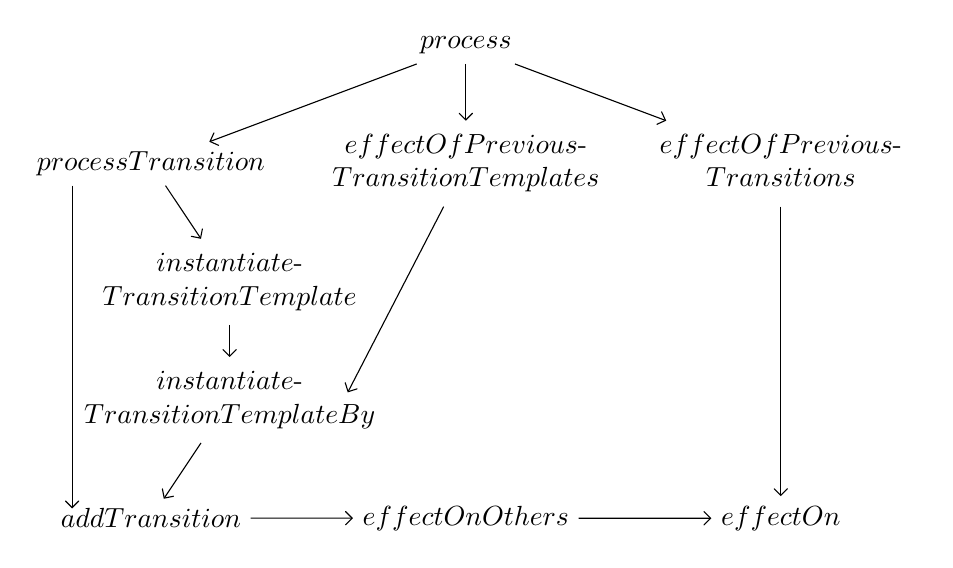
\begin{tikzpicture}[>=angle 90,yscale = 1.5]
\draw (0,0) node (process) {$process$};
\draw (process) ++ (-4,-1) node (processTransition) {$processTransition$};
%
\path[draw,->] (process) -- (processTransition);
\draw (process) ++ (0,-1) node (effectPrevTT)
   {$\begin{array}{c} effectOfPrevious\mbox{-} \\ 
       TransitionTemplates\end{array}$}; 
\path[draw,->] (process) -- (effectPrevTT);
\draw (process) ++ (4,-1) node (effectPrevTrans) 
  {$\begin{array}{c} effectOfPrevious\mbox{-} \\ Transitions\end{array}$}; 
\path[draw,->] (process) -- (effectPrevTrans);
%
\draw (processTransition) ++ (1,-1) node (instantiateTT) 
  {$\begin{array}{c} instantiate\mbox{-}\\ TransitionTemplate \end{array}$};
\path[draw,->] (processTransition) -- (instantiateTT);
%
\draw (instantiateTT) ++ (0,-1) node (instantiateTTBy)
  {$\begin{array}{c} instantiate\mbox{-}\\ TransitionTemplateBy \end{array}$};
\path[draw,->] (instantiateTT) -- (instantiateTTBy);
\path[draw,<-] (instantiateTTBy.north)++(1.5,-0.3) -- (effectPrevTT);
%
\draw (instantiateTTBy) ++ (-1,-1) node (addTransition) {$addTransition$};
\path[draw,->] (instantiateTTBy) -- (addTransition);
\draw (addTransition)++(-1,0) node (addTransitionL) {};
\path[draw,->] (processTransition.south)++(-1,0) -- (addTransitionL);
%
\draw (addTransition) ++ (4,0) node (effectOnOthers) {$effectOnOthers$};
\path[draw,->] (addTransition) -- (effectOnOthers);
%
\draw (effectOnOthers) ++ (4,0) node (effectOn) {$effectOn$}; 
\path[draw,->] (effectOnOthers) -- (effectOn);
\path[draw,->] (effectPrevTrans) -- (effectOn);
\end{tikzpicture}
\end{center}
\caption{Relationship of functions}
\label{fig:impl}
\end{figure}

The function $process(v)$ acts on a single view~$v$ found on the previous ply.
It calculates all the transitions from~$v$, together with the identities of
other components relevant to the view (if any).  It then calls
$processTransition$ on each such transition.  It also calls
$effectOfPreviousTransitions$ and $effect\-Of\-Previous\-TransitionTemplates$
on the view.

The function $processTransition(pre, e, post, ids)$ corresponds to processing
either (1)~the transition $pre \trans{e} post$, if $ids$ is empty, or
(2)~transition template $(pre, post, id, e, true)$ if $ids = \set{id}$,
i.e.~transitions with an extra component with identity~$id$ that synchronises
on~$e$.  It calculates whether the principal component gains a reference to a
component other than those in~$pre$ and~$id$.  If not and $ids$ is empty, the
transition is complete: $addTransition$ is called on it.  Otherwise, it is
added to $newTransitionTemplates$, and
$instantiate\-TransitionTemplate$ is called.

$addTransition(pre,e,post)$ adds a transition $pre \trans{e} post$ to
$new\-Transitions$, and calls $effectOnOthers$.

$effectOnOthers(pre,e,post)$ considers the effect of a new transition $pre
\trans{e} post$ on views found on previous plys.  For each such view that
matches $pre$'s fixed processes, it calls $effectOn$.

$effectOn(pre, e, post, v)$ considers the effect of a transition $pre
\trans{e} post$ on another view~$v$.  It forms all ways of combining $pre$ and
$v$, calculates the corresponding post-view for $v.\princ$, and adds it to
$nextNewViews$.

$instantiateTransitionTemplate(pre, post, id, e, inc)$ considers how to
instantiate the transition template $(pre, post,\linebreak[1] id,\linebreak[1]
e, inc)$.  For each view in $sysAbsViews$ that matches $pre$'s fixed
processes, it calls $instantiate\-Transition\-TemplateBy$.

$instantiateTransitionTemplateBy(pre, post, id, e, inc, v)$ considers how
to instantiate the transition template $(pre, post,\linebreak[1]
id,\linebreak[1] e, inc)$, so that a component of $v$ forms the extra
component with identity~$id$.  For each resulting transition, it calls
$add\-Transition$.

$effectOfPreviousTransitions(v)$ considers the effect of all previous
transitions on a view~$v$ found on the previous ply.  For each
transition in $transitions$ whose initial servers matches $v$'s servers, it
calls $effectOn$.

$effectOfPreviousTransitionTemplates(v)$ considers using a view~$v$ found on
the previous ply to instantiate the missing component in a transition
template.  For each transition template in $transitionTemplates$ whose initial
servers matches $v$'s servers, it calls $instantiateTransitionTemplateBy$.

We briefly discuss the combination of views and either transitions or
transition templates: it is important that we consider each such combination,
just once, regardless of the plys each are found or created on.  Consider a
view~$v$ found on ply~$n$, and expanded on ply~$n+1$.
%
\begin{itemize}
\item On ply~$n+1$, $v$ will be considered (in $effectOfPreviousTransitions$)
  in combination with each transition created up to ply~$n$.

\item For each transition created on ply~$n+1$ or later, its effect on~$v$
  will be considered (in $effectOnOthers$) on the ply in which the transition
  is created. 
 %% A transition from~$v$ will be considered in ply~$n+1$, and its effect
 %%  considered (in $effectOnOthers$) on all views~$v'$ found up to ply~$n$.
\end{itemize}
%
Thus the combination of a view and a transition will be treated: (1)~by the
first bullet if the transition is created on a ply no later than the view is
found; and (2)~by the second bullet if the transition is created on a ply
later than the view is found.  

Likewise
%
\begin{itemize}
\item On ply $n+1$, $v$ will be considered (in
  $effect\-Of\-Previous\-Transition\-Templates$) to create the missing
  component in each transition template created up to ply~$n$.

\item For each transition template created on ply~$n+1$ or later, its
  combination with~$v$ will be considered (in
  $instantiate\-Transition\-Template$) on the ply in which the transition
  template is created.
%% \item A transition template from~$v$ will be created in ply~$n+1$, and all
%%   ways of creating the missing component from views found up to ply~$n$ will
%%   be considered (in $instantiateTransitionTemplate$).
\end{itemize}
%
Thus the combination of a view and a transition template will be treated:
(1)~by the first bullet if the transition template is created on a ply no
later than the view is found; and (2)~by the second bullet if the transition
template is created on a ply later than the view is found.

%%%%%%%%%%%%%%%%%%%%%%%%%%%%%%%%%%%%%%%%%%%%%%%%%%%%%%%

\subsection{instantiateTransitiontemplateBy}

$instantiateTransitionTemplateBy(pre, post, id, e, inc, v)$ considers how
to instantiate the transition template $(pre, post,\linebreak[1]
id,\linebreak[1] e, inc)$, so that a component of $v$ forms the extra
component with identity~$id$.  For each resulting transition, it calls
$add\-Transition$.


The function $consistentStates(pre, id, e, inc, v)$ considers how to rename
$v$ to potentially produce the extra component of the transition template
$(pre, post,\linebreak[1] id,\linebreak[1] e, inc)$.  More precisely, it finds
all ways of renaming~$v$ to obtain a view~$v'$ so that (1) a component of~$v'$
has identity~$id$, (2)~$v'$ and~$pre$ agree on common components, and (3)~if
$inc$ then $v'$ can perform~$e$.  For each, it returns the renamed component
with identity id, and the next states. 

For each such extra component~$st$,\, $isExtendable(pre, st)$ tests whether
$st$ is consistent with $pre$, in the sense that for each component $c$ of
$pre \union st$, the current set of views contains a view with $c$ as
principal component and agreeing on common processes (modulo renaming).

$compatibleWith(servers, components, st)$ tests whether there is an existing
view with $st$ as principal component that agrees with $servers$ and
$components$ on common processes. 

$containsReferencingView(pre, st, j)$ assumes that $pre.components(j)$ has a
reference to $st$.  If tests whether there is a view with $pre.components(j)$
as principal component, containing $st$, and otherwise compatible with~$pre$
(modulo renaming).

*** If the views that ensure consistency are found later, do we get all
instantiations?  I think so.  The last relevant view will include the state we
want. 

\newpage
\subsection{Calculating induced transitions}
\label{sec:induced-symmetry}

We now consider how to calculate the transition induced
by a transition $pre \trans[e] post$ on a view~$v$, given that both are in
normal form and represent all members of their equivalence classes.  
%
Following Definition~\ref{def:induced-transition}, in principle, we need to
find all ways of renaming parameters of~$v$ and~$pre$ to produce views that
are accordant.  However, if two different renamings would produce equivalent
post-views, it is enough to consider just one of them.  It is therefore enough
to keep the parameters of $pre$ fixed, and to rename the parameters of~$v$.
Each renaming can be defined by an renaming~$\pi$ over the parameters of~$v$.
That is, we consider renamings~$\pi$ such that $\pi(v)$ and~$pre$ are
accordant, and consider the effect of the transition on~$\pi(v)$.
%
Below, we restrict the range of such renamings further, while ensuring we
produce a representative of each equivalence class of resulting post-views.



Recall that in order to be accordant, if $\pi(v)$ and $pre$ each have a
component with the same identity, then those components must be equal.  We say
that the renaming has \emph{unified} these components.
%
\begin{definition}
Let $v$ and $pre$ be in normal form.  Then renaming function~$\pi$ over the
parameters of~$v$ is a \emph{unification function} if $\pi(v)$ and $pre$ are
accordant.
%
If $c$ is a component of~$v$, $c'$ is a component of~$pre$, and $\pi(c) = c'$,
we say that $c$ and~$c'$ are \emph{unified}.
\end{definition}
%
Of course, it is possible to unify two components only if they have the same
control state. 

Recall that if $\pi(v)$ and~$pre$ are accordant, then their fixed processes
are equal.  Lemma~\ref{lem:remapping-id-on-fixed-params} then implies that
$v.\fixed = pre.\fixed$ and $\pi$ is the identity over the parameters
of~$v.\fixed$.

%% The following lemma follows from the way we have defined normal
%% forms. 
%% %
%% \begin{lemma}
%% If $v$ and~$pre$ are both in normal form, and $\pi(v)$ and~$pre$ are
%% accordant, then $v.\fixed = pre.\fixed$ and $\pi$ is the identity over the
%% parameters of~$v.\fixed$.
%% \end{lemma}

%%%%%

\begin{example}
We use a running example to illustrate the technique.  Consider
\begin{eqnarray*}
pre & = &
   (fixed(N_0); Th(T_0, N_1, N_2), Nd_A(N_1, N_3), Nd_B(N_2, N_0, N_4)), 
\\
post & = & 
  (fixed'(N_5); Th'(T_0, N_1, N_2), Nd_C(N_1, N_2, N_3), Nd_B(N_2, N_0, N_4)) ,
\\
v & = & 
  (fixed(N_0); Nd_A(N_1, N_2), Nd_B(N_2, N_0, N_3)).
\end{eqnarray*}
%
$pre$ and~$v$ have fixed processes in the same states, so there is the
potential to produce a renaming~$\pi(v)$ accordant with~$pre$.  We start with
the partial renaming function $\pi = \set{N_0 \mapsto N_0}$, the identity over
the parameters of the fixed processes.
%% It is worth noting that the identifiers $N_1$, $N_2$ and~$N_3$ that appear in
%% both~$pre$ and~$v$ might represent different parameters, since each substate
%% is just a representative of its equivalence class.  The fact that the same
%% identifiers appear in each substate is just an artefact of the way we produce
%% normal forms.
\end{example}

%%%%%

In general, any subset of the components of~$v$ might be unified with
components of~$pre$ (including no unifications).  For each potential choice of
which components to unify, we construct the minimal renaming function that
extends the identity function over the parameters of the fixed processes so as
to rename the parameters of each unified component of~$v$ to the parameters of
the corresponding component of~$pre$.  We call the resulting function a
\emph{partial unification function}.  However, some such choices of
unifications might prove impossible, if no such function exists.
%
\begin{definition}
Let $v$ and $pre$ be in normal form with $v.\fixed = pre.\fixed$.  Then a
partial renaming function~$\pi$ is a \emph{partial unification function} if
\begin{itemize}
\item $\pi$ is the identity function over the parameters of $v.\fixed$;

\item $\pi$ is defined over the parameters of a subset of the components
  of~$v$, mapping each such component to unify it with a component of $pre$;

\item $\pi$ is undefined over all parameters not included under the previous
  two points.
\end{itemize}
\end{definition}


%%%%%

\begin{example}
We continue with the running example.  Unifying the two $Nd_A$ processes
gives the partial unification function
%
\begin{eqnarray*}
\pi_1 & = & \set{N_0 \mapsto N_0, N_1 \mapsto N_1, N_2 \mapsto N_3}.
\end{eqnarray*}
%
Alternatively, unifying the two $Nd_B$ processes gives
\begin{eqnarray*}
\pi_2 & = & \set{N_0 \mapsto N_0, N_2 \mapsto N_2, N_3 \mapsto N_4}.
\end{eqnarray*}
It is not possible to unify both pairs simultaneously, since $N_2$ cannot be
mapped consistently.  In addition, the renaming~$\pi$ corresponds to unifying
no components.
\end{example}

We now need to extend each such renaming function in a consistent way.  The
following definition describes what that means.
%
\begin{definition}
\label{def:consistent-extension}
Let $pre \trans[e] post$ be an extended transition, and $v$ be a view, both in
normal form, with $v.\fixed = pre.\fixed$.
%
Consider a partial unification function~$\pi$.  We define an extension~$\pi'$
of~$\pi$ to be a \emph{consistent extension} if (a)~the renaming~$\pi'$ is
injective and defined over all parameters of~$v$; and (b)~whenever a
component~$c$ in~$v$ is not unified with any component of~$pre$, the identity
of~$c$ is not mapped to an identity of a component~$c'$ in~$pre$ (since that
would require unifying~$c$ and~$c'$).
\end{definition}

%%%%%

The following lemma follows directly from the definitions.
%
\begin{lemma}
Let $pre \trans[e] post$ be an extended transition, and $v$ be a view, both in
normal form, with $v.\fixed = pre.\fixed$.  Then every unification
function~$\pi$ is a consistent extension of a partial unification function,
and vice versa.
\end{lemma}

In principal, then, we need to consider all consistent extensions of all
partial unification functions.  However, many different consistent extensions
will end up producing the same new view, up to equivalence, so it will be
enough to build only representative renamings.  Recall
(Definition~\ref{def:induced-transition}) that when we build an induced
transition, the state of each component in the new view is: (1)~the state
from~$post$ for components in the transition; or (2)~the state from~$v$ for
other components.  The unifications already tell us the states in case~(1).
In case~(2), each parameter in the component might or might not be the same as
a parameter taken from $post$.  We need to find all ways of renaming
parameters in such components to give distinct new views, up to equivalence.
The following definition captures the required consistent extensions; we
verify this fact as Proposition~\ref{prop:unifying-renaming}.

%%%%%

\begin{definition}
\label{def:representative-consistent-extension}
Consider an extended transition~$pre \trans[e] post$, a view~$v$, and a
partial unification function~$\pi$.  We define a consistent extension~$\pi'$
of~$\pi$ to be a \emph{representative consistent extension} if for every
parameter~$x$ in~$v$ but not in the domain of~$\pi$,\, $\pi'(x)$ is one of the
following:
%
\begin{enumerate}
\item\label{clause:remap-1} a parameter of $post.\fixed$; 

\item\label{clause:remap-2} a parameter of the state in~$post$ of a unified
  component;

\item\label{clause:remap-3} if the principal of~$v$ is unified with a
  component~$c$, and $c$~gains a reference to a component with identity~$id$,
  then a parameter of the state in~$post$ of~$id$ (note that $pre$ and $post$
  must contain a component with identity~$id$, by
  clause~\ref{assump:secondary-cpts-new-refs} of Assumption~\ref{assump:2}); or

\item\label{clause:remap-4} a minimal fresh parameter, i.e.~a parameter
  different from those in~$pre$ and~$post$, and in each case choosing (in the
  order in which those parameters~$x$ appear in~$v$) the minimal such value
  that hasn't been used previously. 
\end{enumerate}
%
%% Further, under case~\ref{clause:remap-4}, \emph{minimal} fresh parameters are
%% chosen for each such~$x$, in the order in which those parameters~$x$ appear
%% in~$v$ (i.e.~in each case choosing the smallest fresh parameter not already
%% used).
%
Note that these are subject to the conditions~(a) and~(b) of
Definition~\ref{def:consistent-extension}. 
%% These are all subject to two provisos: (a)~that the renaming remains
%% injective; and (b)~a parameter that is the identity of a component~$c$ in~$v$
%% that is not unified with any component of~$pre$ cannot be mapped to an
%% identity of a component in~$pre$ (since that would require unifying~$c$).
\end{definition}
%
%% When a parameter is mapped to a fresh parameter, all choices of the fresh
%% parameter give equivalent post-states.  Hence it is enough to make the choice
%% in one way: we pick the minimal fresh parameter each time. 


%%%%%

\begin{example}
We continue the running example, considering just the unification
corresponding to~$\pi_1$.  Consider what values~$N_3$ can be mapped to.  By
clause~\ref{clause:remap-1}, it can be mapped to~$N_5$.  By
clause~\ref{clause:remap-2}, it can be mapped to~$N_2$.  By
clause~\ref{clause:remap-3}, it can be mapped to~$N_4$ (from the post-state of
the $Nd_B$ process).  Finally, by clause~\ref{clause:remap-4}, it can be
mapped to the minimal fresh value, namely~$N_6$.
%
This then produces four renamings:
\[
\pi_X = \set{N_0 \mapsto N_0, N_1 \mapsto N_1, N_2 \mapsto N_3, N_3 \mapsto X},
\quad \mbox{for $X = N_2, N_4, N_5, N_6$}.
\]
For each such renaming~$\pi_X$,\, $v$ gets remapped to a view of the form
\[
(fixed(N_0); Nd_A(N_1, N_3), Nd_B(N_3, N_0, X)).
\]
The $fixed$ and $Nd_A$ processes evolve under the transition \( pre
\trans{} post \), and the latter gains a reference to~$N_2$ in
$post$.  This produces the four views
\[
(fixed'(N_5); Nd_C(N_1, N_2, N_3), Nd_B(N_2, N_0, N_4), Nd_B(N_3, N_0, X)).
\]
Finally, these views need to be reduced to normal form.  Note that the four
normal forms are distinct.
\end{example}

%%%%%

The following proposition shows that considering representative consistent
extensions is enough to produce all induced transitions, up to equivalence. 
%
\begin{prop}
\label{prop:unifying-renaming}
Consider an extended transition $pre \trans[e] post$ and a view~$v$, both in
normal form, with $v.\fixed = pre.\fixed$.  Consider also a partial
unification function~$\pi$.
%
Let $\pi'$ be a consistent extension of~$\pi$, and
let $v'$ be the view produced by Definition~\ref{def:induced-transition}
considering the effect of $pre \trans[e] post$ on~$\pi'(v)$.  
%
Then there is a representative consistent extension~$\pi''$ of~$\pi$, such
that, letting $v''$ be the view produced by
Definition~\ref{def:induced-transition} considering the effect of $pre
\trans[e] post$ on~$\pi''(v)$, we have $v'' \equiv v'$.
\end{prop}

%%%%%%

\begin{proof}
Let $pre$, $post$, $v$, $\pi$, $\pi'$ and~$v'$ be as in the statement of the
lemma.  We describe how to construct the renaming~$\pi''$, and a
renaming~$\hat\pi$ such that $\pi' = \hat\pi \circ \pi''$.  This will imply
that $\hat\pi(v'') = v'$.  The following figure illustrates (and acts as an
aide-m\'emoire).
%
\begin{center}
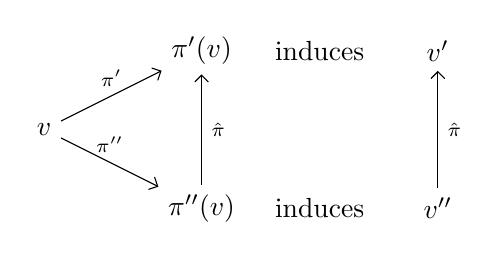
\begin{tikzpicture}[>= angle 90]
\draw (0,0) node (v) {$v$};
%
\draw (2,1) node (pi'v) {$\pi'(v)$};
\path[draw, ->] (v) -- node[above]{\scriptsize $\pi'$} (pi'v);
%
\draw (2,-1) node (pi''v) {$\pi''(v)$};
\path[draw, ->] (v) -- node[above]{\scriptsize $\pi''$} (pi''v);
\path[draw, ->] (pi''v) -- node[right]{\scriptsize $\hat\pi$} (pi'v);
%
\draw (pi'v)++(1.5,0) node (induces1) {induces};
\draw (induces1)++(1.5,0) node (v') {$v'$};
%
\draw (pi''v)++(1.5,0) node (induces2) {induces};
\draw (induces2)++(1.5,0) node (v'') {$v''$};
\path[draw, ->] (v'') -- node[right]{\scriptsize $\hat\pi$} (v');
\end{tikzpicture}
\end{center}
%
In fact, $\hat\pi$ will be the identity over all parameters except for fresh
parameters chosen under clause~\ref{clause:remap-4} of
Definition~\ref{def:representative-consistent-extension}.

We define $\pi''$ as an extension of~$\pi$.  This implies that $\pi''$
and~$\pi'$ agree on values in the domain of~$\pi$, and unify the same
components.  For all values~$y$ in the range of~$\pi$, we define $\hat\pi(y) =
y$. 

Recall that $v'.\fixed = v''.\fixed = post.\fixed$; each component of~$v'$ is
taken from~$post$ if the corresponding component of~$\pi'(v)$ is in~$pre$, and
otherwise is taken from~$\pi'(v)$; and each component of~$v''$ is taken
from~$post$ if the corresponding component of~$\pi''(v)$ is in~$pre$, and
otherwise is taken from~$\pi''(v)$.  We arrange for~$v'$ and~$v''$ to take the
same components from~$post$.

%% For each parameter~$x$ of~$v.\fixed$, we define $\pi''(x) = x$.  This means
%% $\pi''(v).\fixed = pre.fixed$.  And we define $\hat\pi(x) = x$. 

For each parameter~$x$ of~$v$ such that $y = \pi'(x)$ is a parameter of
$post.\fixed$, we define $\pi''(x) = y$, and $\hat\pi(y) = y$.  Note that each
such value~$y$ is included under case~\ref{clause:remap-1} of
Definition~\ref{def:representative-consistent-extension}.  This ensures
that~$\pi''(v)$ and~$\pi'(v)$ agree on all such~$y$; and hence~$v'$ and~$v''$
agree on all such~$y$.  Note that this is a consistent extension of~$\pi$,
because~$\pi'$ is a consistent extension of~$\pi$.  

For each parameter~$x$ such that $y = \pi'(x)$ is a parameter of a component
of~$v'$ taken from~$post$, we again define $\pi''(x) = y$, and $\hat\pi(y) =
y$.  Note that each such value $y$ is included under
case~\ref{clause:remap-2} or \ref{clause:remap-3} of
Definition~\ref{def:representative-consistent-extension}.  This ensures
that~$\pi''(v)$ and~$\pi'(v)$ agree on all such~$y$; and hence~$v'$ and~$v''$
agree on all such~$y$; in particular, they include the same components taken
from~$post$.  Again note that this is a consistent extension of~$\pi$,
because~$\pi'$ is a consistent extension of~$\pi$. 

Finally, each other parameter~$y$ in~$v'$ must necessarily be in a component
taken from~$\pi'(v)$.  Suppose the parameter is $\pi'(x)$, and $x$ is not in
the domain of~$\pi$.  We define $\pi''(x)$ to be the minimal fresh
parameter~$z$, chosen as in
Definition~\ref{def:representative-consistent-extension}; and we let
$\hat\pi(z) = y$.  This ensures that $v''$ uses~$z$ wherever $v'$ uses~$y$.
Also note that this is a consistent extension of~$\pi$, by construction.
\end{proof}

%%%%%

\begin{impNote}
\texttt{Unification.combine} produces the remapped version of~$v$, together
with information about the unifications.  If uses \texttt{allUnifs} to find
all choices of unification and corresponding renaming function~$\pi$.  Then
\texttt{extendUnif} extends this, and produces the remapped state.

\texttt{EffectOn.apply} produces the corresponding post-views.
\end{impNote}

%%%%%

\subsubsection{Optimisations} 


%%%%%

\begin{opt}
Recall Optimisation~\ref{opt:avoid-induced}.  
\begin{itemize}
\item For case~\ref{case:avoid-induced-1}, we avoid unifying the principal
  of~$v$ with the principal of~$pre$.

\item For case~\ref{case:avoid-induced-2}, if $pre.\fixed = post.\fixed$ we
  require that at least one component of~$v$ unifies with a component that
  changes state.

\item For case~\ref{case:avoid-induced-3}, we store a record of pairs
  $(v, post.\fixed)$ for which we have considered the effect of a transition
  $pre \trans[e] post$ on~$v$ for which $pre.\fixed \ne post.\fixed$,\,
  %% $unifs$ describes which components of~$v$ unify with which components
  %% of~$pre$ (
  and $v$
  unifies with no component.
%
  If subsequently we consider a similar case ---that is, the same
  $post.\fixed$ and~$v$, and no unifications--- we identify that it will not
  produce any new views, and so avoid the construction.
\end{itemize}
\end{opt}


\begin{impNote}
Done in isSufficientUnif. 
\end{impNote}

\begin{improve}
The third case is not quite the same as in
Optimisation~\ref{opt:avoid-induced}.  There we included cases where $pre$
and~$v$ shared a component that did not change state.  An obvious attempt to
implement this goes wrong: if there are two cases with the same $post.\fixed$
and~$v$, that include unifications of \emph{different} components that do not
change state, they might give different new views (with the unified components
having different parameters in $post.\fixed$).
%
For example
\begin{eqnarray*}
pre & = & (fixed; Th_1(T_0,N_0), Nd_A(N_0,N_1)) \\
post & = & (fixed'(N_1); Th_1'(T_0), Nd_A(N_0,N_1)) \\
v & = & (fixed; Th_v(T_0,N_0), Nd_A(N_0,N_1))
\end{eqnarray*}
unifying the two $Nd_A$ processes, with remapping $\set{T_0 \mapsto T_1, N_0
  \mapsto N_0,\linebreak[1] {N_1 \mapsto N_1}}$, induces
\[
(fixed'(N_1); Th_v(T_1,N_0), Nd_A(N_0,N_1) \equiv
(fixed'(N_0); Th_v(T_0,N_1), Nd_A(N_1,N_0)).
\]
But with 
\begin{eqnarray*}
pre' & = & (fixed; Th_2(T_0,N_0,N_1), Nd_A(N_0,N_2), Nd_N(N_1,Null)) \\
post' & = & (fixed'(N_1); Th_2'(T_0), Nd_A(N_0,N_2), Nd_N(N_1,Null))
\end{eqnarray*}
unifying the two $Nd_A$ processes, with remapping $\set{T_0 \mapsto T_1, N_0
  \mapsto N_0,\linebreak[1] {N_1 \mapsto N_2}}$, induces a transition to
\[\mit
(fixed'(N_1); Th_v(T_1,N_0), Nd_A(N_0,N_2)) \equiv
  (fixed'(N_0); Th_v(T_0,N_1), Nd_A(N_1, N_2)).
\]


If we have two cases concerning the same $post.\fixed$, $v$, and component~$c$
of~$v$ that unifies and doesn't change state, and $c$ unifies respectively
with~$c_1$ and~$c_2$ which differ only on parameters not in $post.\fixed$,
then it is enough to consider just one such case.  In the above example, we
had $c_1 = Nd_A(N_0,N_1)$,\, $c_2 = Nd_A(N_0,N_2)$ which differ on~$N_1$. 

\framebox{Do this.}  For the components, it's enough to store the list of
parameters shared with $post.\fixed$ and their indices. 
\end{improve}

 
%%%%%%%%%%%%%%%%%%%%

\begin{opt}
If the principal of~$v$ is unified with a component of~$pre$, and loses a
reference to a component~$c$, then all renamings of~$c$ produce the same final
view.  Thus it is enough to consider a single renaming, say the renaming that
agrees with the renaming within other components, but otherwise maps to fresh
parameters.  There is no need to explicitly construct the renaming of~$c$.  
%
\framebox{Consider this.}

This won't work with singleRef, however, because of cross references or
missing references. 
\end{opt}

%%%%%

\begin{improve} 
If the principal and another component~$c$ of~$v$ are both unified with
components of $pre$, and the principal of~$v$ loses the reference to~$c$ in
the transition, then for case~\ref{clause:remap-2} of
Definition~\ref{def:representative-consistent-extension}, we can ignore
parameters of~$c$.  This is only relevant for renaming of some third
component.
%
This might be useful when a node has a reference to the thread, but loses
that reference.
\end{improve}


%%%%%%%%%%%%%%%%%%%%%%%%%%%%%%%%%%%%%%%%%%%%%%%%%%%%%%%


\end{document}
